%%%%%%%%%%%%%%%%%%%%%%%%%%%%%%%%%%%%%%%%%%%%%%%%%%%%%%%%%%%%%%%%%%%%%%%%%%%%%%%%%%
\begin{frame}[fragile]\frametitle{}
\begin{center}
{\Large Random Variables}
\end{center}
\end{frame}

%%%%%%%%%%%%%%%%%%%%%%%%%%%%%%%%%%%%%%%%%%%%%%%%%%%%%%%%%%
\begin{frame}\frametitle{Random Variables}
\begin{itemize}
\item Those variables which can take different value randomly are called
random variables.
\item If the variables are discrete in nature, they are called discrete random
variables.
\item Similarly, if the variables are continuous in nature, then it is called
continuous random variable.
\end{itemize}
\end{frame}



%%%%%%%%%%%%%%%%%%%%%%%%%%%%%%%%%%%%%%%%%%%%%%%%%%%%%%%%%%
\begin{frame} \frametitle{Random variables}
A {\bf random variable} is generated by a ``random'' function. 

Types:
\begin{itemize}
\item Nominal
\item Ordinal
\item Quantitative
\end{itemize}
\end{frame}


%%%%%%%%%%%%%%%%%%%%%%%%%%%%%%%%%%%%%%%%%%%%%%%%%%%%%%%%%%
\begin{frame}\frametitle{Nominal Random Variable}
\begin{itemize}
\item A {\bf nominal} random variable, also called {\bf qualitative} or {\bf  categorical}, takes on values in a set of names or labels.
\item Examples of nominal sample spaces include geographical locations, biological species, and ethnic categories.
\item Data from a nominal random variable cannot be {\bf strictly ordered}.
\end{itemize}
\end{frame}

%%%%%%%%%%%%%%%%%%%%%%%%%%%%%%%%%%%%%%%%%%%%%%%%%%%%%%%%%%
\begin{frame}\frametitle{Ordinal Random Variable}

\begin{itemize}
\item An {\bf ordinal} measurement is usually either a {\bf ranking}
($1^{\rm st}$, $2^{\rm nd}$, etc.) or a {\bf rating} (good, bad,
favorable, strongly agree, etc.).  

\item Ordinal values can be ordered, but do not have {\bf measurement units}
\item It doesn't always make sense to subtract or divide their numerical
values.
\end{itemize}
\end{frame}

%%%%%%%%%%%%%%%%%%%%%%%%%%%%%%%%%%%%%%%%%%%%%%%%%%%%%%%%%%
\begin{frame}\frametitle{Quantitative Random Variable}

\begin{itemize}
\item A {\bf quantitative} random variable represents a magnitude, for
example the result of counting something, or the result of measuring a
physical quantity such as length, width, or volume.

\item Quantitative measurements can always be ordered.
\end{itemize}
\end{frame}

%%%%%%%%%%%%%%%%%%%%%%%%%%%%%%%%%%%%%%%%%%%%%%%%%%%%%%%%%%%
%\begin{frame}
%\frametitle{Measurement scales}
%
%\begin{itemize}
%\item Celsius temperature is an interval scale -- it makes
%perfect sense to compare two temperatures by subtracting them.
%\item Is Celsius temperature a ratio scale?  Is the coffee twice as hot as
%the tea?
%\item 
%The answer is no.  The freezing point of water defines the origin of
%the Celsius scale.  This is arbitrary.  Pure ethanol freezes at
%$-114^\circ$C, so if we used the freezing point of ethanol as the zero
%point of the scale, the ratio between the two objects' temperatures
%would be only $(50+114)/(25+114)=1.2$.
%
%\textcolor{blue}{Note:} There is some ambiguity and controversy about
%these designations.
%
%\end{frame}

%%%%%%%%%%%%%%%%%%%%%%%%%%%%%%%%%%%%%%%%%%%%%%%%%%%%%%%%%%%
\begin{frame}
\frametitle{ Quantitative Random Variable }
Types:
\begin{itemize}
\item Discrete: Number of days that it rains yearly 
\item Continuous:  Amount of rain on a given day 
\end{itemize}
Note that these designations aren't used in the case of nominal or
ordinal random variables.
\end{frame}

%%%%%%%%%%%%%%%%%%%%%%%%%%%%%%%%%%%%%%%%%%%%%%%%%%%%%%%%%%%
\begin{frame}
\frametitle{ Quantitative Random Variable }

\begin{itemize}
\item A {\bf discrete} random variable takes on finitely many values, or
infinitely many separated values (e.g.\ $0,1,2,\ldots$).

\item A {\bf continuous} random variable can take on any real number in some
interval (e.g.\ $[0,1]$ or $[0,\infty)$).  

\item Gray area between discrete and continuous random variables:
e.g.\ monetary values recorded in dollars or dollars and cents
\end{itemize}
\end{frame}

%%%%%%%%%%%%%%%%%%%%%%%%%%%%%%%%%%%%%%%%%%%%%%%%%%%%%%%%%%%
\begin{frame}
\frametitle{Units, populations and samples}

\begin{itemize}
\item A {\bf unit} (more specifically {\bf ``sampling unit''}) is one member
of the collection.
\item A {\bf population} is the set of all units of interest. 
\item In practice, we cannot observe the whole population, so we usually
work with a {\bf sample} of units
\end{itemize}
\end{frame}

%%%%%%%%%%%%%%%%%%%%%%%%%%%%%%%%%%%%%%%%%%%%%%%%%%%%%%%%%%%
\begin{frame}
\frametitle{Units, populations and samples}

%\textcolor{blue}{\bf Example:} Suppose we are interested in childrens'
%diets, and we sample 100 seven year old
%girls in the US and record their food intake for one day.

\begin{itemize}
\item Properties of a sample will generally differ from properties of the
population.  
\item For example, the 100 children in our sample may have
somewhat higher or somewhat lower average calorie intake than the
population at large. 
\item 
Statistics: how samples relate to
populations, and what we can confidently state about a population
given the limited information in a sample.

\end{itemize}

\end{frame}

%%%%%%%%%%%%%%%%%%%%%%%%%%%%%%%%%%%%%%%%%%%%%%%%%%%%%%%%%%
\begin{frame}\frametitle{Random Variables}
\begin{itemize}
\item  Random variable can take on randomly different
value. 
\item But are all the values that it takes can be equal or likely be equal
too, or is it more likely that the random variable take a particular value
more often than other?
\item Depends on the way (function) using which random numbers are generated.
\end{itemize}
\end{frame}

%%%%%%%%%%%%%%%%%%%%%%%%%%%%%%%%%%%%%%%%%%%%%%%%%%%%%%%%%%
\begin{frame}\frametitle{Random Variable Generation}
\begin{itemize}
\item  Experiment: records numbers from a SINGLE six face die.
\item X axis shows 6 possible outcomes.
\item Y axis shows their probabilities.
\item For each of the 6 possible values on X axis, the Y value is same ie 1/6
\item Uniform distribution
\end{itemize}
\end{frame}

%%%%%%%%%%%%%%%%%%%%%%%%%%%%%%%%%%%%%%%%%%%%%%%%%%%%%%%%%%
\begin{frame}\frametitle{Random Variable Generation}
\begin{itemize}
\item  Experiment: records sum of numbers from TWO six face dies.
\item X axis shows 12 possible outcomes.
\item Y axis shows their probabilities.
\item For each of the 12 possible values on X axis, the Y value is NOT SAME.
\end{itemize}

\begin{center}
\includegraphics[width=0.5\linewidth,keepaspectratio]{pmf}
\end{center}
\end{frame}

%%%%%%%%%%%%%%%%%%%%%%%%%%%%%%%%%%%%%%%%%%%%%%%%%%%%%%%%%%
\begin{frame}\frametitle{Random Variable Generation}
\begin{itemize}
\item  If the random variable is discrete in nature, we use Probability Mass
Function to describe its probability distribution
\item If the random variable is continuous in nature, we use Probability
Density Function to describe its probability distribution.
\end{itemize}
\end{frame}

%%%%%%%%%%%%%%%%%%%%%%%%%%%%%%%%%%%%%%%%%%%%%%%%%%%%%%%%%%%
\begin{frame}
\frametitle{Probability distributions}
The probability distribution for a random variable X gives the possible 
values for X, and the probabilities associated with each possible value 
(i.e., the likelihood that the values will occur). 
Types:
\begin{itemize}
\item Discrete probability distributions 
\item Continuous probability distributions 
\end{itemize}
\end{frame}

%%%%%%%%%%%%%%%%%%%%%%%%%%%%%%%%%%%%%%%%%%%%%%%%%%%%%%%%%%%
\begin{frame}
\frametitle{Discrete Probabilities}

\begin{itemize}
\item If a random variable has a discrete sample space, a probability
distribution is just a listing of the probabilities with which each
point in the sample space occurs.  
\item These probabilities must sum to 1.
\end{itemize}
\end{frame}


%%%%%%%%%%%%%%%%%%%%%%%%%%%%%%%%%%%%%%%%%%%%%%%%%%%%%%%%%%%
\begin{frame}
\frametitle{Example: Discrete Probabilities}

\begin{itemize}
\item Survey of a political candidate.  

\begin{center}
\begin{tabular}{ll}
{$x$} & {$P(X=x)$}\\\hline Favorable & \hspace{0.8cm}0.3 \\ Neutral
& \hspace{0.8cm}0.5 \\ Unfavorable & \hspace{0.8cm}0.2 \\\hline
\end{tabular}
\end{center}

\item
The mapping from points in a discrete sample space to the
corresponding probabilities is called a {\bf probability mass function
  (PMF)}.
\item
The sample space is finite.
\end{itemize}
\end{frame}

%%%%%%%%%%%%%%%%%%%%%%%%%%%%%%%%%%%%%%%%%%%%%%%%%%%%%%%%%%%
\begin{frame}
\frametitle{Many Discrete Probabilities}

\begin{itemize}
\item Infinitely many
rows

\begin{center}
\begin{tabular}{ll}
{$x$} & {$P(X=x)$}\\\hline 
0 & \hspace{0.8cm}0.37\\
1 & \hspace{0.8cm}0.37\\
2 & \hspace{0.8cm}0.18\\
3 & \hspace{0.8cm}0.06\\
$\cdots$ & \hspace{0.8cm}$\cdots$
\end{tabular}
\end{center}
\item 
Although there are infinitely many nonzero probabilities, they still
must sum to one.
\end{itemize}
\end{frame}
%
%
%%%%%%%%%%%%%%%%%%%%%%%%%%%%%%%%%%%%%%%%%%%%%%%%%%%%%%%%%%%%
%\begin{frame}
%\frametitle{Example: Many Discrete Probabilities}
%
%\begin{itemize}
%\item Suppose we flip a coin repeatedly until
%we get the first tail, and count the number of heads that we see
%before the tail occurs.  
%\item The sample space is $\{0,1,2,\ldots\}$ -- it
%is infinite.
%\end{itemize}
%\end{frame}

%%%%%%%%%%%%%%%%%%%%%%%%%%%%%%%%%%%%%%%%%%%%%%%%%%%%%%%%%%%
\begin{frame}
\frametitle{Probability Mass Function }

\begin{itemize}
\item function that generates discrete variables with probabilities
\item $f(x_i) = P(X=x_i)$ is the probability that $X$ has the value $x_i$.
\item Properties:
\begin{itemize}
\item $0\leq f(x_i)\leq1 $
\item $\sum f(x_i) =f(x_1) +f(x_2) + \ldots = 1$ 
\end{itemize}
\end{itemize}
\end{frame}

%%%%%%%%%%%%%%%%%%%%%%%%%%%%%%%%%%%%%%%%%%%%%%%%%%%%%%%%%%%
\begin{frame}
\frametitle{Example: Probability Mass Function }

\begin{itemize}
\item Suppose the random variable X is the number of rooms in a 
randomly chosen owner-occupied housing unit. 
\item The distribution of X is: 

\begin{center}
\includegraphics[width=0.8\linewidth,keepaspectratio]{rooms}
\end{center}
\end{itemize}

\end{frame}


%%%%%%%%%%%%%%%%%%%%%%%%%%%%%%%%%%%%%%%%%%%%%%%%%%%%%%%%%%%
\begin{frame}
\frametitle{Probability Density Function }

\begin{itemize}
\item function that generates continous random variables with probabilities
\item $f(x_{(a,b)}) = P(X=x_{(a,b)})$ is the probability that $X$ has the values in range $(a,b)$.
\item Properties:
\begin{itemize}
\item $0\leq f(x_i)\leq1 $
\item $\int f(x_i) = 1$ 
\end{itemize}
\end{itemize}
\end{frame}

%%%%%%%%%%%%%%%%%%%%%%%%%%%%%%%%%%%%%%%%%%%%%%%%%%%%%%%%%%%%
\begin{frame}
\frametitle{Distributions of continuous random variables}

Two important identities are

\begin{center}
\begin{tabular}{ccc}
$P(X>x)$ &=& $1 - P(X \le x)$\\ $P(a < X \le b)$ &=& $P(X\le b) -
  P(X < a)$.
\end{tabular}
\end{center}

Therefore we only need to know $P(X \le x)$ for all values of $x$ and
we can determine the probability that $X$ lies in any given interval.

{\bf Its area under curve}
\end{frame}

%%%%%%%%%%%%%%%%%%%%%%%%%%%%%%%%%%%%%%%%%%%%%%%%%%%%%%%%%%%%
\begin{frame}
\frametitle{Distributions of continuous random variables}

\textcolor{blue}{\bf Example:} Suppose we want to know the probability
that a person in a certain population is between 170cm and 180cm tall.
If we know that the probability of being less than 180cm tall is
$0.8$, and the probability of being less than 170cm tall is $0.6$,
then the probability of being between 170cm and 180cm tall is
$0.8-0.6=0.2$.

To put this in mathematical notation, let $X$ denote the height of a
randomly selected person from the population.  Then 

$$ P(170<X\le 180) = P(X\le 180) - P(X<170) = 0.8-0.6.
$$

\end{frame}

%%%%%%%%%%%%%%%%%%%%%%%%%%%%%%%%%%%%%%%%%%%%%%%%%%%%%%%%%%%
\begin{frame}
\frametitle{Density functions}

The distribution of a continuous random variable is described by a
{\bf density function}.  

A density function is a non-negative function such that the area
between the horizontal axis and the function is exactly 1.

The orange curves below are density functions.  The grey area on the
left is $P(X \le -0.5)$, which is 0.31 for this distribution.  The
grey area on the right is $P(X \le 2.5)$, which is 0.92 for this
distribution.


% \begin{center}
% \begin{tabular}{cc}
% \scalebox{0.4}{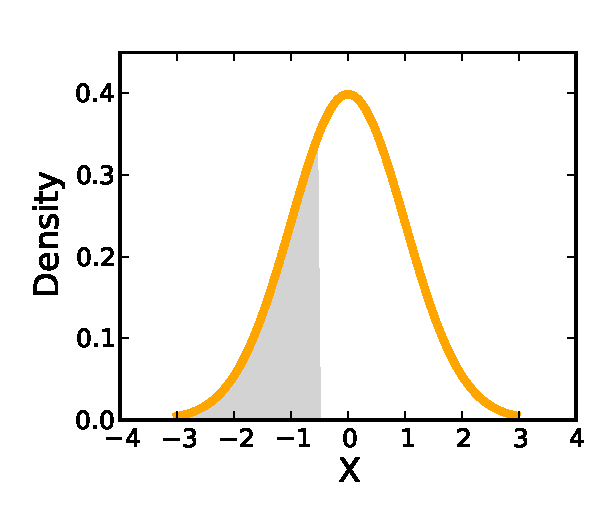
\includegraphics{000.pdf}} &
% \scalebox{0.4}{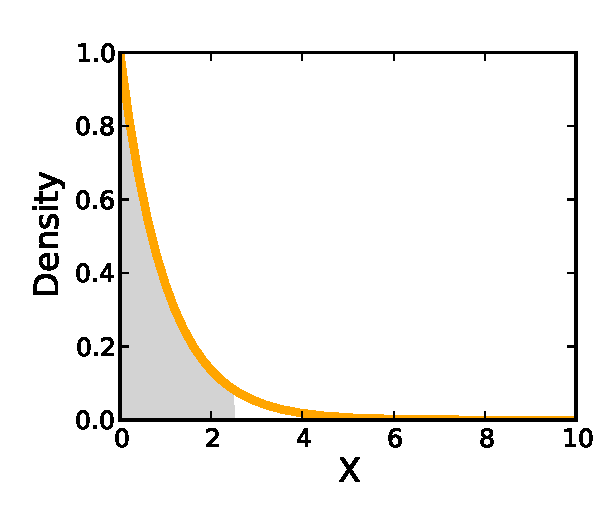
\includegraphics{001.pdf}}
% \end{tabular}
% \end{center}

\end{frame}

%%%%%%%%%%%%%%%%%%%%%%%%%%%%%%%%%%%%%%%%%%%%%%%%%%%%%%%%%%%
\begin{frame}
\frametitle{Characteristics of density functions}

A basic property of a density function is its {\bf location} -- the
central or most typical value.  

There are many measures of location, but by any reasonable measure the
density on the right, below, would have a greater location than the
density on the left.

% \begin{center}
% \begin{tabular}{cc}
% \scalebox{0.4}{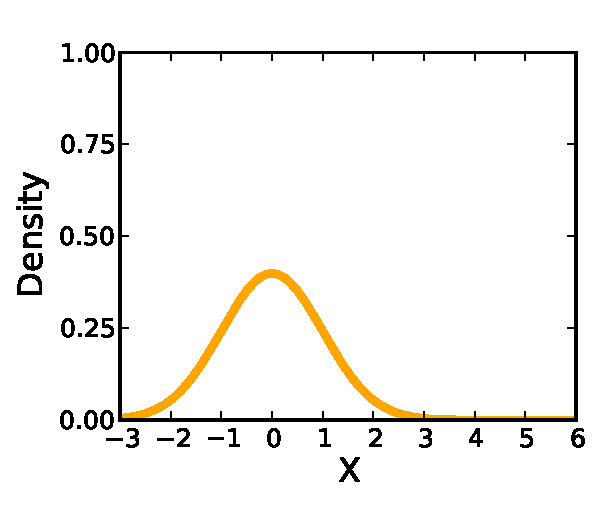
\includegraphics{002-0.pdf}}&
% \scalebox{0.4}{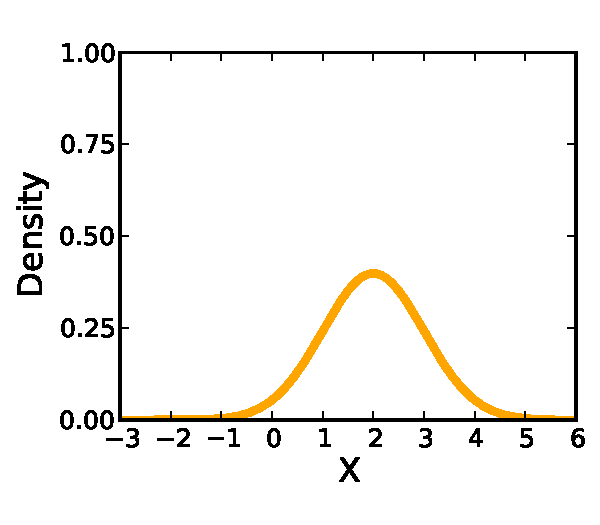
\includegraphics{002-1.pdf}}
% \end{tabular}
% \end{center}

\end{frame}

%%%%%%%%%%%%%%%%%%%%%%%%%%%%%%%%%%%%%%%%%%%%%%%%%%%%%%%%%%%
\begin{frame}
\frametitle{Characteristics of density functions}

Another basic property of a density function is its {\bf scale},
referring to spread or width of the distribution.  

There are many measures of scale, but by any reasonable measure the
density on the right, below, would have a greater scale than the
density on the left.

% \begin{center}
% \begin{tabular}{cc}
% \scalebox{0.4}{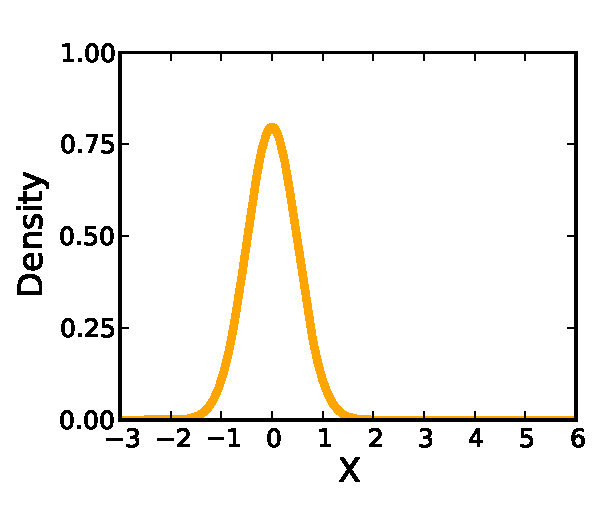
\includegraphics{002-2.pdf}}&
% \scalebox{0.4}{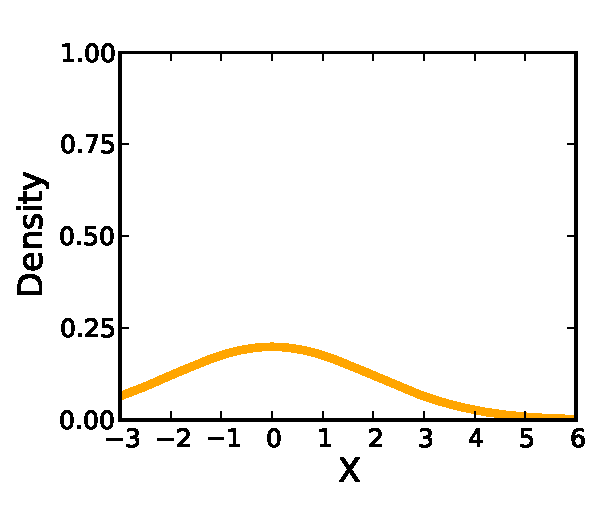
\includegraphics{002-3.pdf}}
% \end{tabular}
% \end{center}


\end{frame}

%%%%%%%%%%%%%%%%%%%%%%%%%%%%%%%%%%%%%%%%%%%%%%%%%%%%%%%%%%%
\begin{frame}
\frametitle{Characteristics of density functions}

Another basic property of a density function is its {\bf skew},
referring to whether one of the two tails of the density is thicker
than the other.  

The density on the left, below, is right-skewed, and the density on
the right, below, is left-skewed.


% \begin{center}
% \begin{tabular}{cc}
% \scalebox{0.4}{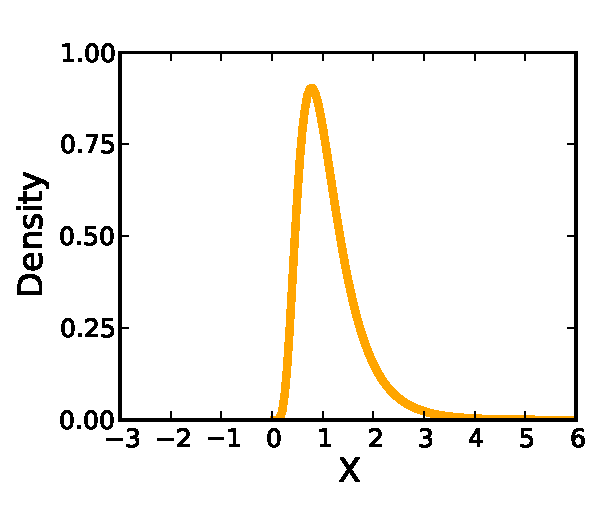
\includegraphics{002-4.pdf}}&
% \scalebox{0.4}{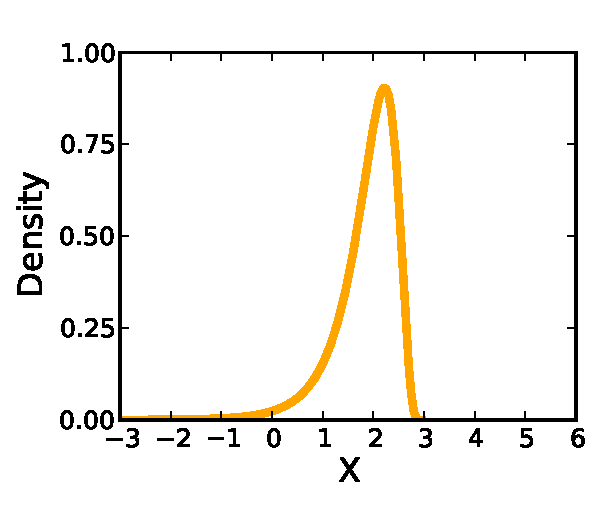
\includegraphics{002-5.pdf}}
% \end{tabular}
% \end{center}

%The densities on the preceding two slides are unskewed, or symmetric.

\end{frame}


%%%%%%%%%%%%%%%%%%%%%%%%%%%%%%%%%%%%%%%%%%%%%%%%%%%%%%%%%%%
\begin{frame}
\frametitle{Discrete Probability Distributions }
Some examples:
\begin{itemize}
\item Bernoulli distribution :$ P(X = 1) = p,           P(X = 0) = 1- p$
 
\item Binomial distribution : -Two possible outcomes, probability constant = $(\frac{n}{x})p^x (1-p)^{n-x}$
 
\item Poisson distribution 
 
\item Negative Binomial 
\end{itemize}
\end{frame}

%%%%%%%%%%%%%%%%%%%%%%%%%%%%%%%%%%%%%%%%%%%%%%%%%%%%%%%%%%
\begin{frame}{Bernoulli}

Bernoulli random variable is used when the experiment results in
either success or failure where success is represented as 1 and failure as
0. If P is probability of success, then probability mass function of
Bernoulli variable x is given as:

\begin{center}
\includegraphics[width=0.45\linewidth,keepaspectratio]{bernoulli}
\end{center}
\end{frame}

%%%%%%%%%%%%%%%%%%%%%%%%%%%%%%%%%%%%%%%%%%%%%%%%%%%%%%%%%%
\begin{frame}{Binomial}

Binomial distribution is used when we want to count how many success we
have when we repeat an experiment for n numbers of time
independently. The probability mass function of binomial variable x,
where p is probability of success, is given as:

\begin{center}
\includegraphics[width=0.45\linewidth,keepaspectratio]{binom}
\end{center}
\end{frame}

%%%%%%%%%%%%%%%%%%%%%%%%%%%%%%%%%%%%%%%%%%%%%%%%%%%%%%%%%%
\begin{frame}{Poisson}

Poisson variable x is used when we are counting the number of
occurrences of an event in a unit of time such that the occurrences are
independent and rarely simultaneous. For an average number of
occurrence $\lambda$ the probability mass function is given as:
\begin{center}
\includegraphics[width=0.45\linewidth,keepaspectratio]{poisson}
\end{center}
\end{frame}


%%%%%%%%%%%%%%%%%%%%%%%%%%%%%%%%%%%%%%%%%%%%%%%%%%%%%%%%%%%
\begin{frame}
\frametitle{Continuous Probability Distributions }
Some examples:
\begin{itemize}
\item  Normal distribution 
 
\item  Uniform distribution 
 
\item  Exponential distribution 
 
\item  Weibull distribution 
 
\end{itemize}
\end{frame}

%%%%%%%%%%%%%%%%%%%%%%%%%%%%%%%%%%%%%%%%%%%%%%%%%%%%%%%%%%
\begin{frame}{Normal}

Normal random variable x comes handy for different situations. We can
use it to model physical measurements like weight, height etc. We can
also use it to model error made by measuring instruments. In general, it
can be used when the average and variance of the quantity being
measured is known. The probability density function is given as:
\begin{center}
\includegraphics[width=0.65\linewidth,keepaspectratio]{normdist1}
\end{center}
\end{frame}

%%%%%%%%%%%%%%%%%%%%%%%%%%%%%%%%%%%%%%%%%%%%%%%%%%%%%%%%%%
\begin{frame}{Uniform}

We use uniform random variable x when the probability density for
every value between an interval (starting from a and ending at b) is
equal. The probability density function of x is given as:
\begin{center}
\includegraphics[width=0.65\linewidth,keepaspectratio]{uniform}
\end{center}
\end{frame}

%%%%%%%%%%%%%%%%%%%%%%%%%%%%%%%%%%%%%%%%%%%%%%%%%%%%%%%%%%
\begin{frame}{Exponential}

Exponential variable x are used when we are measuring the time until
the  rst occurrence of an event, such that the occurrences in disjoint
time intervals are independent and rarely simultaneous. For the
average number of occurrences per unit time a, the probability density
function is given as:
\begin{center}
\includegraphics[width=0.65\linewidth,keepaspectratio]{expo}
\end{center}
\end{frame}

%%%%%%%%%%%%%%%%%%%%%%%%%%%%%%%%%%%%%%%%%%%%%%%%%%%%%%%%%%%
\begin{frame}
\frametitle{Event probabilities}

An {\bf event} is a set of one or more points in the sample space.
The probability of an event is the sum of the probabilities for the
points in the event.

\textcolor{blue}{\bf Example:} Consider this distribution:

\begin{center}
\begin{tabular}{ll}
{$x$} & {$P(X=x)$}\\\hline 
Favorable & \hspace{0.8cm}0.3 \\
Neutral & \hspace{0.8cm}0.5 \\
Unfavorable & \hspace{0.8cm}0.2 \\\hline
\end{tabular}
\end{center}

The response being either \textcolor{purple}{favorable or neutral} is
an event, and this event has probability $0.3+0.5=0.8$.

\end{frame}

%%%%%%%%%%%%%%%%%%%%%%%%%%%%%%%%%%%%%%%%%%%%%%%%%%%%%%%%%%%
\begin{frame}
\frametitle{Cumulative probabilities}

If the sample space is ordered, then the probability of observing a
value less than or equal to a given number $x$ is the {\bf cumulative
  probability at $x$}.

\textcolor{blue}{\bf Example:} If we are interested in the probability
distribution of the number of times a person living in Michigan has
visited Florida, we might have the following probabilities and
cumulative probabilities:

\begin{center}
\begin{tabular}{lllllllll}
$x$         & 0   & 1 & 2 & 3 & 4 & 5 & $\cdots$\\\hline
$P(X=x)$    & 0.3 & 0.1 & 0.2 & 0.1 & 0.06 & 0.08 & $\cdots$\\
$P(X\le x)$ & 0.3 & 0.4 & 0.6 & 0.7 & 0.76 & 0.84 & $\cdots$\\\hline
\end{tabular}
\end{center}

\end{frame}

%%%%%%%%%%%%%%%%%%%%%%%%%%%%%%%%%%%%%%%%%%%%%%%%%%%%%%%%%%%%
%\begin{frame}
%\frametitle{Exercises}
%
%The following distribution describes the number of times a 20 year-old
%male visits a doctor in a year.  Some of the probabilities are not
%shown.
%
%\begin{center}
%\begin{tabular}{lllll}
%$x$         & 0   & 1 & 2 & 3+ \\\hline
%$P(X=x)$    & 0.55 & ? & 0.1 & ?\\
%\end{tabular}
%\end{center}
%
%\begin{itemize}
%
%\item What is the range of possible values for the probability that
%  exactly one visit to the doctor occurs?
%
%\item What are the largest and smallest possible values for the
%  cumulative probability at 1?
%
%\item What are the largest and smallest possible values for the
%  probability that the person visits the doctor at least
%  once?
%
%\end{itemize}
%
%\end{frame}

%%%%%%%%%%%%%%%%%%%%%%%%%%%%%%%%%%%%%%%%%%%%%%%%%%%%%%%%%%%
\begin{frame}
\frametitle{Independence}

Two random variables are {\bf independent} if the probability that
both of them satisfy some condition at the same time is the product of
the probabilities of the conditions being satisfied separately.

For example,

$$
P(X=2\;{\rm and}\;Y=3) = P(X=2)\cdot P(Y=3)
$$

\begin{center}
$P(0\le X<1\;{\rm and}\;Y>4) = P(0 \le X < 1)\cdot P(Y>4)$ 
\end{center}

\end{frame}

%%%%%%%%%%%%%%%%%%%%%%%%%%%%%%%%%%%%%%%%%%%%%%%%%%%%%%%%%%%
\begin{frame}
\frametitle{Example: Independence}

\begin{itemize}
\item College students at an educational institution where 52\% of the
students are female,
\item 40\% of the students visit a doctor at
least once a year.

\item the probability
that a randomly selected student is female and has visited a doctor in
the last year is?

\item  $0.52\times 0.4 = 0.208$.

\item Corollary: if the value sis not $0.208$ then these variables
are {\bf dependent}.
\end{itemize}
\end{frame}

%%%%%%%%%%%%%%%%%%%%%%%%%%%%%%%%%%%%%%%%%%%%%%%%%%%%%%%%%%%
\begin{frame}
\frametitle{Independence}
\begin{itemize}

\item If the proportion is greater than 0.208, the variables are {\bf
  positively dependent}.

\item If the proportion is less than 0.208, the variables are {\bf
  negatively dependent}.

\end{itemize}

\end{frame}
%
%%%%%%%%%%%%%%%%%%%%%%%%%%%%%%%%%%%%%%%%%%%%%%%%%%%%%%%%%%%%
%\begin{frame}
%\frametitle{Independence}
%
%\textcolor{blue}{\bf Example:} suppose we are interested in the
%relationship between a person's income at age 30 (denoted $I$), and
%the number of siblings they have (denoted $S$).  If these two random
%variables are independent, then
%
%\begin{eqnarray*}
%P(I=\$45,000\;{\rm and}\; S=1) &=& P(I=\$45,000)\times P(S=1)\\
%P(I=\$55,000\;{\rm and}\; S=2) &=& P(I=\$55,000)\times P(S=2)
%\end{eqnarray*}
%
%The multiplication property holds for all events, not just events
%consisting of a single outcome.  If $I$ and $S$ are independent, then
%
%\begin{eqnarray*}
%\lefteqn{P(\$35,000 \le I \le \$55,000\; {\rm and}\; S\le 1) =}\\ 
%&&P(\$35,000 \le I \le \$55,000)\times P(S\le 1).
%\end{eqnarray*}
%
%\end{frame}

%%%%%%%%%%%%%%%%%%%%%%%%%%%%%%%%%%%%%%%%%%%%%%%%%%%%%%%%%%%%
\begin{frame}
\frametitle{Complements}

\begin{itemize}

\item For a particular event $E$, there is a related event denoted $E^c$
which is the event that $E$ does not happen.

\item Example: $E$ may be that the person who answers is female.  
\item The complementary
event would be the event that the person who answers is male.

\item The probability of the complement of an event is 1 minus the
probability of the event: $P(E^c) = 1 - P(E)$.
\end{itemize}


\end{frame}

%%%%%%%%%%%%%%%%%%%%%%%%%%%%%%%%%%%%%%%%%%%%%%%%%%%%%%%%%%%%
\begin{frame}
\frametitle{Complements}
\textcolor{blue}{\bf Example:} If the probability that a person
living in Michigan has visited Florida at most two times is 0.6, the
complementary event is that the person has visited Florida three or
more times, and the probability of this event is 0.4.
% \begin{center}
% \begin{tabular}{cc}
% \scalebox{0.4}{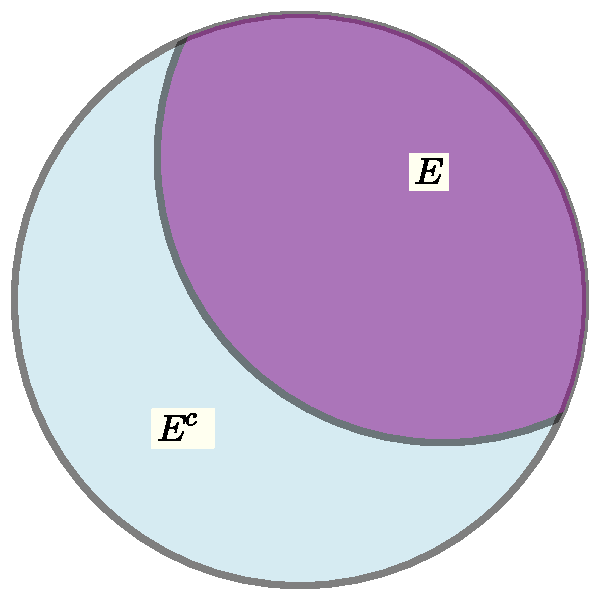
\includegraphics{039-1.pdf}}&
% \scalebox{0.4}{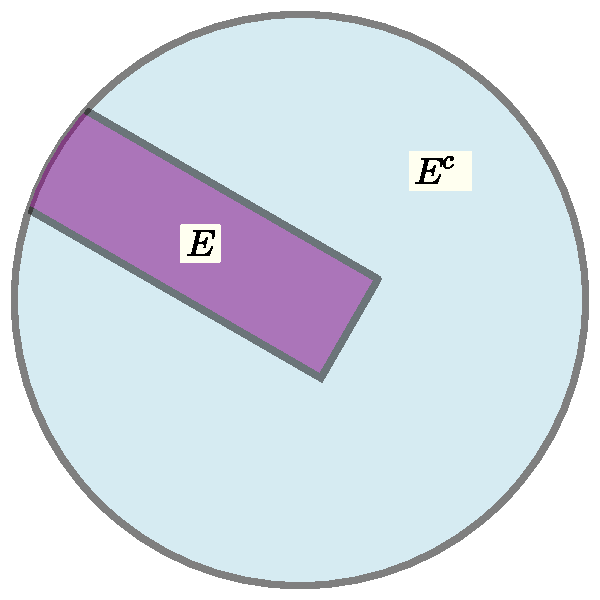
\includegraphics{039-2.pdf}}
% \end{tabular}
% \end{center}

\end{frame}

%%%%%%%%%%%%%%%%%%%%%%%%%%%%%%%%%%%%%%%%%%%%%%%%%%%%%%%%%%%%
\begin{frame}
\frametitle{Disjoint events}

Two events are {\bf disjoint} if they contain no points in common.
These two events are disjoint:

\begin{center}
\begin{tabular}{ll}
E1:& A person's birthday is on the 31st day of the month\\
E2:& A person's birthday is in June
\end{tabular}
\end{center}

\end{frame}

%%%%%%%%%%%%%%%%%%%%%%%%%%%%%%%%%%%%%%%%%%%%%%%%%%%%%%%%%%%%
\begin{frame}
\frametitle{Disjoint events}

But these events are not disjoint:

\begin{center}
\begin{tabular}{ll}
E1:& A person's birthday is on a Tuesday\\
E2:& A person's birthday is in June
\end{tabular}
\end{center}

\end{frame}

%%%%%%%%%%%%%%%%%%%%%%%%%%%%%%%%%%%%%%%%%%%%%%%%%%%%%%%%%%%%
\begin{frame}
\frametitle{Disjoint events}

Events $E1$ and $E2$ are disjoint on the left, but not on the
right. The large gray circle represents the full sample space.

% \begin{center}
% \begin{tabular}{cc}
% \scalebox{0.4}{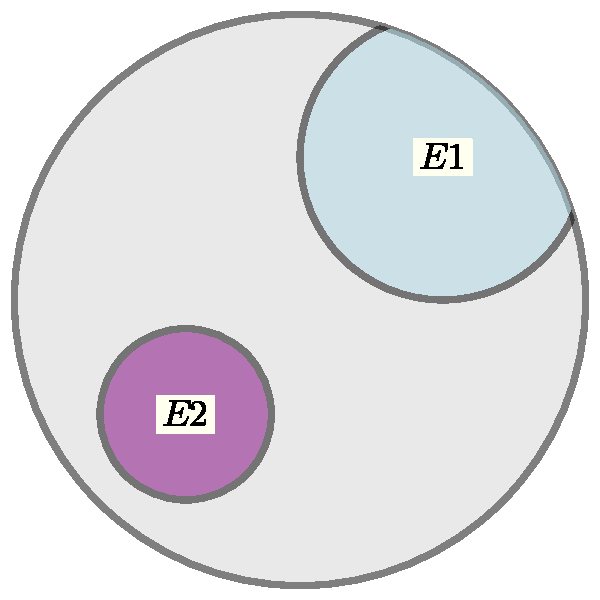
\includegraphics{040-1.pdf}}&
% \scalebox{0.4}{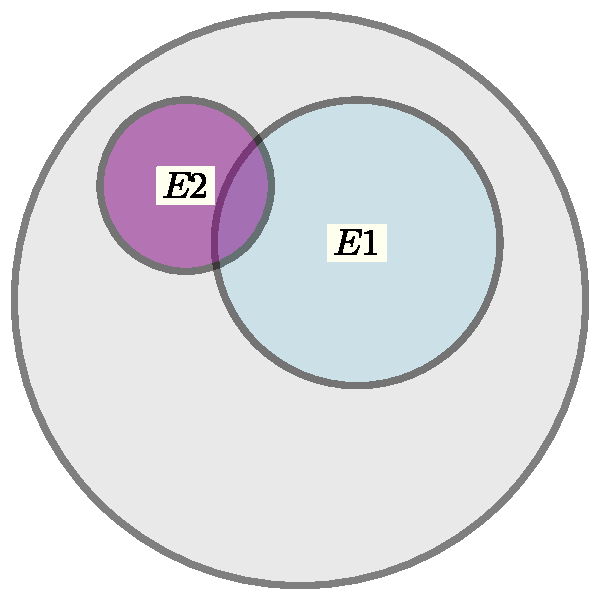
\includegraphics{040-2.pdf}}
% \end{tabular}
% \end{center}

\end{frame}


%%%%%%%%%%%%%%%%%%%%%%%%%%%%%%%%%%%%%%%%%%%%%%%%%%%%%%%%%%%%
\begin{frame}
\frametitle{Disjoint events}

If events $E1$ and $E2$ are disjoint, then the probability of at least
one of them happening is the sum of their probabilities:

$$
P(E1\;{\rm or}\;E2) = P(E1) + P(E2).
$$
\end{frame}

%%%%%%%%%%%%%%%%%%%%%%%%%%%%%%%%%%%%%%%%%%%%%%%%%%%%%%%%%%%%
\begin{frame}
\frametitle{Example: Disjoint events}
Roll a fair die, and consider these events:

\begin{center}
\begin{tabular}{ll}
E1:& The result is even\\
E2:& The result is a 3 or a 5
\end{tabular}
\end{center}

The event ``$E1$ or $E2$'' is the event that I get a 2, 3, 4, 5, or 6.
This event has probability $5/6$.  Since $P(E1) = 1/2$ and $P(E2) =
1/3$, we can check that $P(E1\;{\rm or}\;E2) = 5/6 = 1/2 + 1/3 = P(E1)
+ P(E2)$.

\end{frame}

%%%%%%%%%%%%%%%%%%%%%%%%%%%%%%%%%%%%%%%%%%%%%%%%%%%%%%%%%%%%
\begin{frame}
\frametitle{Disjoint events}

Now consider these events:

\begin{center}
\begin{tabular}{ll}
E1:& The result is even\\
E2:& The result is less than or equal to 3
\end{tabular}
\end{center}

These events are not disjoint, since 2 is in both events.

The event ``$E1$ or $E2$'' is the event that I get a 1, 2, 3, 4, or 6.
This event has probability $5/6$.  But $P(E1) = 1/2$ and $P(E2) = 1/2$
so $P(E1)+P(E2) \ne P(E1\;{\rm or}\;E2)$.

\end{frame}

%%%%%%%%%%%%%%%%%%%%%%%%%%%%%%%%%%%%%%%%%%%%%%%%%%%%%%%%%%%%
\begin{frame}
\frametitle{Exercises}

Suppose we are considering a population of students that is 52\%
female, and for which 40\% of the students have visited a doctor in
the last year.

\begin{itemize}

\item If these events are independent, what is the probability that a
  randomly sampled student is a male who has not seen a doctor in the
  last year?

\item If these events are independent, what is the probability that a
  randomly sampled student is either a male who has not seen a doctor
  in the last year, or is a female who has not seen a doctor in the
  last year?

\item If there are 1000 students in our population, and gender is
  independent of whether a student visited a doctor in the past year,
  how many students are females who have not seen a doctor in the past
  year?

\end{itemize}

\end{frame}

%%%%%%%%%%%%%%%%%%%%%%%%%%%%%%%%%%%%%%%%%%%%%%%%%%%%%%%%%%%%
\begin{frame}
\frametitle{Answers}


\begin{itemize}

\item $P(Student=Male) = 0.48$, and $P(StudentNoSeenDoctorLastYear) = 0.6$ (both are complements of the events given in the exercise).  By
  independence, $P(Student=Male,And,StudentNoSeenDoctorLastYear) = 0.48*0.6 = 0.288$.

\item Simalalry $P(Student=Female,And,StudentNoSeenDoctorLastYear) = 0.52*0.6 =
  0.312$.  These events are disjoint, so the probability of one or the
  other occuring is 0.288+0.312 = 0.6.  It's not a coincidence that
  this is equal to 1-0.4, the probability of visiting a doctor
  regardless of gender.

\item The probability that a student is a female who has not seen a
  doctor in the last year is 0.312, so the number of such people is
  1000*0.312 = 312.

\end{itemize}

\end{frame}

%%%%%%%%%%%%%%%%%%%%%%%%%%%%%%%%%%%%%%%%%%%%%%%%%%%%%%%%%%%%%%
%%\begin{frame}
%%\frametitle{Distributions of continuous random variables}
%%
%%\begin{itemize}
%%
%%\item For a continuous random variable, $P(X=x)=0$ for all $x$.  
%%
%%\item It takes on values in an interval, for example
%%
%%$$
%%P(X\le 3),\; P(X>-1),\; P(2 < X \le 3).
%%$$
%%
%%\end{itemize}
%%\end{frame}


